Problem synchronizowania silników elektrycznych znany jest w~dziedzinie automatyki od dziesiątek lat. Początki badania silników sięgają XIX wieku, kiedy to Michael Faraday oraz inni naukowcy eksperymentowali ze wykorzystaniem elektromagnetyzmu\cite{bib:pierwszesilniki}. Pierwsze silniki elektryczne były prymitywne i~nie miały zaawansowanych metod sterowania. Wczesne próby pozycjonowania opierały się głównie na prostych mechanizmach, takich jak przekładnie i~sprzęgła.

W miarę postępu technologicznego, szczególnie w~XX wieku, rozwijano bardziej zaawansowane metody pozycjonowania. Pojawiły się pierwsze systemy sterowania, wykorzystujące technologię zwrotną informacji, mającą na celu monitorowanie i~regulację położenia wałów silników. Jednak precyzja tych rozwiązań była ograniczona, a~dokładność pozycjonowania nie zawsze spełniała wymagania coraz bardziej zaawansowanych zastosowań.

Dopiero wprowadzenie enkoderów (Definicja~\ref{def:enkoder}) elektronicznych w~latach 60.~XX~wieku\cite{bib:pierwszeenkodery} stało się przełomem.

\begin{Definition}[Enkoder obrotowy]\label{def:enkoder}
    Urządzenie, generujące sygnały elektryczne odpowiadające ruchowi obrotowemu wału silnika celem określenia jego pozycji. 
\end{Definition}

Początkowo enkodery były oparte na szczotkach stykających się z dyskiem zawierającym serię odpowiednio zakodowanych pierścieni koncentrycznych (Rysunek~\ref{fig:encoderDiscAbsolute}), wypełnionych otworami o odpowiedniej długości\cite{bib:rodzajeenkoderow}. Są one tanie w~produkcji, jednak mają swoje ograniczenia związane ze zużyciem mechanicznym elementów stykowych, niską maksymalną dozwoloną prędkością silnika i~wymaganiami konserwacji. Ten typ enkoderów spotykany jest do dziś, na przykład w multimetrach cyfrowych.

Rozwój technologii przyniósł enkodery optyczne, wykorzystujące diody LED i~fotodetektory. Później pojawiły się enkodery magnetyczne. To właśnie one --- enkodery optyczne i~magnetyczne --- są do dnia dzisiejszego najczęściej spotykane i~oferują najwyższą dokładność sterowania przy niskich kosztach i~niewielkim stopniu skomplikowania. To właśnie na nich skupiono się w~dalszej części pracy.

Enkodery można podzielić ze względu na\cite{bib:rodzajeenkoderow}:
\begin{itemize}
    \item Metodę używaną do odczytania pozycji: kontaktowe i~bezkontaktowe.
    \item Rodzaj sygnału wyjściowego: pozycja absolutna lub szereg inkrementujących/dekrementujących wartości.
    \item Zjawisko fizyczne wykorzystane do przesłania sygnału pozycyjnego: przewodzenie elektryczne, magnetyzm, zjawiska optyczne lub pojemnościowe.
\end{itemize}

Najważniejszy jest podział ze względu na rodzaj sygnału wyjściowego. Mimo, że zarówno enkodery absolutne jak i~inkrementalne posiadają dyski kodujące, różnią się one działaniem. Enkodery absolutne jako sygnał wyjściowy podają precyzyjną pozycję wału silnika, najczęściej zakodowaną w~słowie bitowym. Przykładowy wygląd dysku kodującego widoczny jest na Rysunku~\ref{fig:encoderDiscAbsolute}. Istotną cechą tego rodzaju enkoderów jest możliwość określenia pozycji nawet po utracie zasilania.

\begin{center}
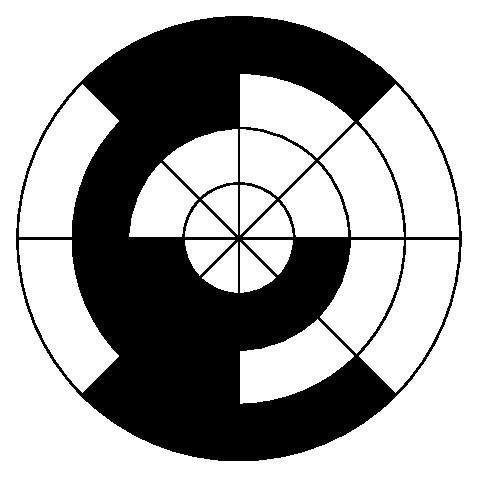
\includegraphics[scale=1]{images/encoderDiscAbsolute.eps}
\captionof{figure}{Poglądowy schemat dysku enkodera absolutnego z 3-bitowym kodem Graya\cite{bib:tarczaenkoderaabsolutnego}.}
\label{fig:encoderDiscAbsolute}
\end{center}

Enkodery inkrementalne u~podstaw działają~w ten sam sposób, tzn. opierają się na dyskach kodujących, z~tą różnicą, że nie są w~stanie podać dokładnej wartości położenia. Zamiast tego, podają na wyjściu odpowiedni impuls przy obrocie w~danym kierunku. Następnie w~oprogramowaniu impulsy te są zliczane w celu oszacowania aktualnej pozycji względem pozycji startowej. Ze względu na wyzerowanie liczby impulsów przy utracie zasilania, ten typ enkodera nie jest w~stanie podać dokładnej pozycji w~przypadku utraty zasilania.

Istotny jest również podział enkoderów ze względu na wykorzystywane zjawisko fizyczne. Dwa główne typy to enkodery optyczne oraz magnetyczne. Pierwszy rodzaj występuje zarówno w~wariancie pojedynczym (Rysunek~\ref{fig:encoderDiscIncrementalSingle}) jak i~podwójnym (Rysunek~\ref{fig:encoderDiscIncrementalDual}). Drugi zaś, ze względu na występowanie polaryzacji biegunów, jedynie w~wariancie pojedynczym (Rysunek~\ref{fig:encoderDiscIncrementalSingle}). W~przypadku enkoderów optycznych, kolorowi białemu odpowiada szczelina, zaś kolorowi czarnemu blokada. W~przypadku enkoderów optycznych, kolorom odopowiadają bieguny~S~i~N.

\begin{figure}
    \centering
    \subfloat[Enkoder pojedynczy]{
      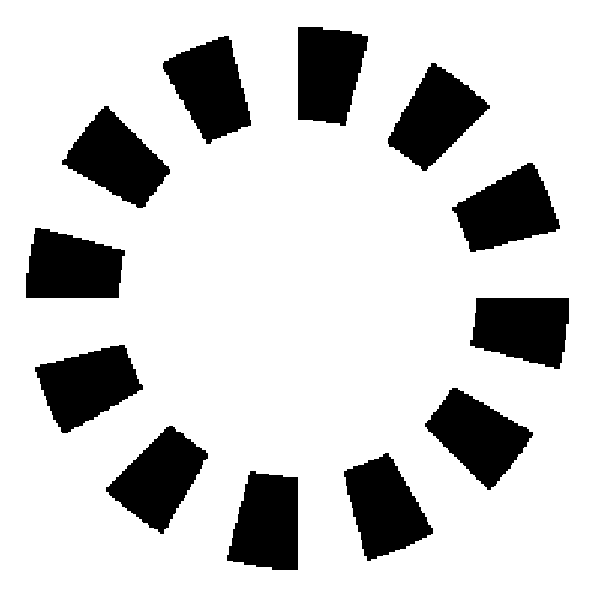
\includegraphics[width=6cm]{images/encoderDiscIncrementalSingle.eps}
      \label{fig:encoderDiscIncrementalSingle}
    }\qquad
    \subfloat[Enkoder podwójny (kwadratowy)]{
      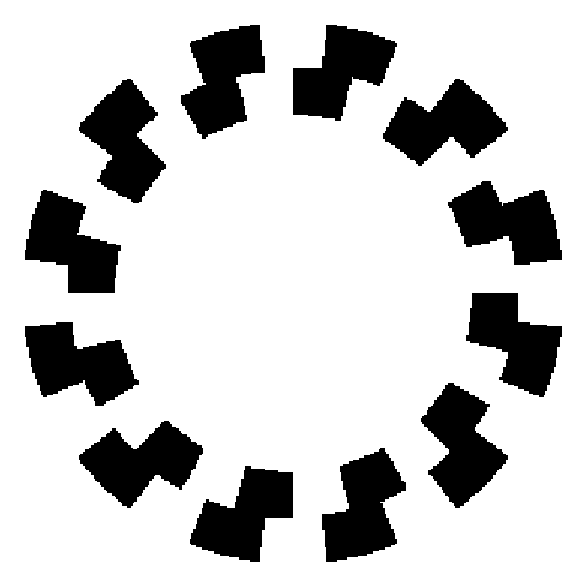
\includegraphics[width=6cm]{images/encoderDiscIncrementalDual.eps}
      \label{fig:encoderDiscIncrementalDual}
    }
    \caption{Poglądowe schematy dysku enkodera \cite{bib:tarczeenkoderowinkrementalnych}}
\end{figure}